\documentclass[12pt]{article}

\usepackage[spanish]{babel}
\usepackage{hyperref}
\usepackage{graphicx}
\usepackage{listings}
\usepackage{color}
\usepackage{multicol}
\usepackage{amssymb}
\spanishdecimal{.}
\usepackage{enumitem}
\usepackage{here}
%% Título
\title{Matemáticas para las Ciencias Aplicadas I}

%% Fecha
\date{\today}

%% Autor
\author{Flores Morán Julieta Melina \\ Zarco Romero José Antonio}


%% Se marca el inicio del documento.
\begin{document}

%% Comando para crear el título.
\maketitle

\section{La edad de la sábana santa}
Zarco Romero José Antonio\\

\begin{figure}[h]
\centering
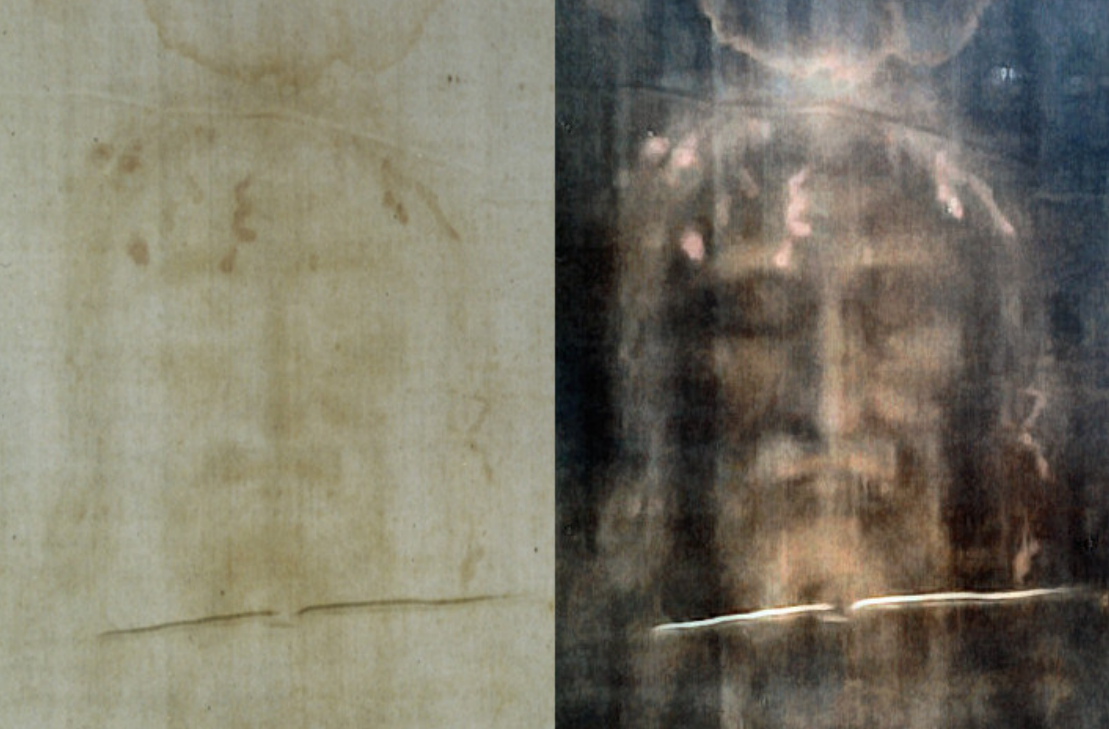
\includegraphics[width=0.7\textwidth]{img/sabanaSanta.png}
\end{figure}
Figura 1: La sábana de Turín: foto moderna de la cara; el positivo a la izquierda y la imagen digitalmente procesada, a la derecha.\\

En 1988, el Vaticano autorizó que el Museo Británico datara la reliquia conocida como la sábana de Turín, posiblemente el sudario del entierro de Jesús de Nazareth. La sábana tiene impresa la imagen de un cuerpo humano que fue venerada como la de Jesús, aunque en la misma Iglesia católica ha habido controversias respecto a su autenticidad. Los resultados del Museo Británico mostraron que el contenido de carbono 14 de la sábana estaba entre el $92 \%$ y el $93 \%$ del correspondiente a una tela recién hecha. Con base en esta información y el dato de que la vida media del carbono 14 es de aproximadamente 5730 años:

\begin{enumerate}	
\item Calcule la cantidad de carbono 14 que debería haberse encontrado en la sábana de Turín en 1988, si hubiera sido tejida en tiempos de Jesús.

Para resolver el problema debemos conocer la fórmula para calcular la cantidad del Carbono 14
\[
C_{14}=f(t)=a_1 \cdot e^{-a_2 \cdot t}
\]
donde $a_1$ y $a_2$ son constantes. En este caso, $a_1$ es la cantidad inicial de Carbono 14 (expresada en porcentaje)
\[
C_{14}=f(t)=100 \cdot e^{-a_2 \cdot t}
\]
Para calcular el valor de la constante $a_2$, utilizaremos el dato de la vida media, el cual expresa lo siguiente $f(5730)=\frac{100}{2}$. Por lo que
\[
\frac{100}{2}=100 \cdot e^{-a_2 \cdot 5730}
\]
\[
\frac{1}{2}=e^{-a_2 \cdot 5730}
\]
\[
ln(\frac{1}{2}) = ln ( e^{-a_2 \cdot 5730} )
\]
\[
ln(2^{-1}) = ln ( e^{-a_2 \cdot 5730} )
\]
\[
-ln(2) = -a_2 \cdot 5730
\]
\[
ln(2) = a_2 \cdot 5730
\]
\[
a_2 = \frac{ln(2)}{5730}
\]
Sustituyendo $a_2$ en la fórmula original, nuestra fórmula para calcular la cantidad del Carbono 14 en base al tiempo queda de la siguiente manera
\[
C_{14}=f(t)=100 \cdot e^{-\frac{ln(2)}{5730} \cdot t}
\]
Si $t=1988$
\[
f(1988)=100 \cdot e^{-\frac{ln(2)}{5730} \cdot 1988}
\]
\[
f(1988)=100 \cdot e^{-0.24048}
\]
\[
f(1988)=100 \cdot 0.78624
\]
\[
\therefore C_{14}=f(1988)=78.624\%
\]
La cantidad de Carbono 14 que debería haberse encontrado en la sábana de Turín en 1988, si hubiera sido tejida en tiempos de Jesús, sería de 78.624\%

\item Explique por qué los arqueólogos del Museo Británico dictaminaron que la tela del sudario debió haberse tejido entre 1299 y 1380.

Ahora, debemos interesarnos en encontrar la función inversa $f^{-1}$ de $C_{14}=f(t)=100 \cdot e^{-\frac{ln(2)}{5730} \cdot t}$. Así, podremos calcular el tiempo transcurrido en base a los porcentajes $92\%$ y $93\%$ de Carbono 14 obtenidos por el Museo Británico.
Para esto, resolveremos la ecuación para t en términos de $C_{14}$
\[
C_{14}=100 \cdot e^{-\frac{ln(2)}{5730} \cdot t}
\]
\[
\frac{C_{14}}{100}=e^{-\frac{ln(2)}{5730} \cdot t}
\]
\[
ln(\frac{C_{14}}{100})=ln(e^{-\frac{ln(2)}{5730} \cdot t})
\]
\[
ln(\frac{C_{14}}{100})=-\frac{ln(2)}{5730} \cdot t
\]
\[
\therefore t =-\frac{5730 \cdot ln(\frac{C_{14}}{100})}{ln(2)}
\]

Si $C_{14}=92$, entonces el tiempo transcurrido en años sería de
\[
t =-\frac{5730 \cdot ln(\frac{92}{100})}{ln(2)}=689.28595
\]
Así, el año cuando debió habese tejido la sábana sería
\[
1988-689.28595=1298.71404
\]
Si $C_{14}=93$, entonces el tiempo transcurrido en años sería de
\[
t =-\frac{5730 \cdot ln(\frac{93}{100})}{ln(2)}=599.91597
\]
Así, el año cuando debió habese tejido la sábana sería
\[
1988-599.91597=1388.08402
\]
$\therefore$ En caso al procentaje $C_{14}=92$, se tiene que el sudario debió haberse tejido alrededor del año 1298.71404. A su vez, si $C_{14}=93$, se tiene que el sudario debió haberse tejido alrededor del año 1388.08402

\item Dé su opinión sobre la siguiente afirmación: “únicamente un milagro explicaría que la imagen impresa en la sábana de Turín sea la de Jesús de Nazareth”.

Desde una perspectiva científica, basada en los avances tecnológicos, concluimos en los apartados anteriores que la sábana de Turín no puede ser el auténtico sudario del entierro de Jesús de Nazareth, ya que la prueba de carbono-14 indica que fue tejido entre los años 1299 y 1380.

Por lo tanto, la afirmación de que solo un milagro podría explicar la imagen en la Sábana de Turín es una declaración basada en la fe y la interpretación personal.

\end{enumerate}



\section{La malahora del occiso}
Flores Morán Julieta Melina\\
\\
Según la \textit{ley de enfriamiento de Newton}, si un cuerpo con temperatura inicial $T (0) = T_0$ se
sumerge en un medio cuya temperatura ambiente $T_a$ permanece constante, donde $T_0 > T_a$, la
temperatura $T(t)$ del cuerpo en el momento $t$ viene dada por la función: \\
(1)\\
\[
T(t)= T_a + (T_0-T_a)e^{-kt},
\]
donde k es una constante positiva.\\ 

El cadáver de una víctima de asesinato es descubierto a la media noche y, en ese momento,
el médico forense registra que la temperatura del cuerpo es de $31  ^{\circ} C$ y, una hora más tarde, la temperatura del cadáver es de $29  ^{\circ} C $. 
Si se supone que la temperatura del aire circundante permanece constante a $21 ^{\circ}  C$ y que la temperatura "normal" de un ser humano vivo es de $37  ^{\circ} C$, con base en estos datos y la ley de enfriamiento de Newton, calcular la hora en que ocurrió el asesinato. Para ello, siga este procedimiento:
\begin{enumerate}
\item Suponga que $t = 0$ es el momento en que se encuentra el cadáver. Identifique los valores
correspondientes a $T_0$ y $T_a$ de este problema y sustitúyalos en la ecuación (1) para obtener
que, en este caso:
\[
T_0 = Temperatura \;a \;la\; media \;noche= 31  ^{\circ} C
\]
\[
T_a = Temperatura \;del \;ambiente = 21 ^{\circ}  C
\]
Remplazando estos valores se tiene que : 
\[
T(t)= 21 + (31-21)e^{-kt}
\]
(2)
\[
\therefore  T(t)= 21 + 10e^{-kt}
\]  
\item Para determinar el valor de $-k$, tome en cuenta que $T(1) = 29$, sustituya $t = 1$ en la ecuación (2) y despeje $k$ para mostrar que:
\[
 T(1)= 21 + 10e^{-k} = 29
\]  
\[
 10e^{-k} = 29-21
\]  
\[
  e^{-k} = \frac{8}{10}
\]  
\[
 -k = ln\frac{8}{10}
\]  
\[
 \therefore  k = -ln\frac{8}{10} = 0.2231435513
\] 
\item Sustituya el valor de $-K$ en la ecuación (2) para obtener la ecuación de enfriamiento del
cadáver:\\
(3)
\[
T(t)= 21 + 10e^{-0.2231435513t}
\] 
\item Por último, use el dato de que en el momento de la muerte, la víctima tenía una temperatura
corporal de $37  ^{\circ} C$ para concluir que el asesinato ocurrió a las 21 : 54 horas; es decir, dos horas y seis minutos antes de la media noche.
\\
Para conocer el tiempo transcurrido dada una temperatura, necesitamos la inversa de esta función, la cual tendrá como variable independiente la temperatura y como variable dependiente el tiempo transcurrido. \\
Despejamos t para conocer la inversa de: 
\[
T= 21 + 10e^{-0.2231t}
\] 
Entonces
\[
\frac{T-21}{10}= e^{-0.2231t}
\] 
\[
ln \frac{T-21}{10}= -0.2231t
\] 
\[
t = -ln \frac{T-21}{10} \times \frac{1}{0.2231}
\]
\[
\therefore T^{-1}(t) = -ln \frac{t-21}{10} \times \frac{1}{0.2231}
\]
$T^{-1}$ es la función inversa, dada una t que es la temperatura de la que se quiere saber el tiempo transcurrido.\\
Para  $37  ^{\circ} C$:
\[
T^{-1}(37) = -ln \frac{37-21}{10} \times \frac{1}{0.2231} = -2.106694
\]
Este resultado indica que los $37  ^{\circ} C$ fue la temperatura de cuerpo 2.106694 horas antes de $T_0$ que se tomó a la media noche.\\
Considerando que:
\[
	0.106694\;h \;(\frac{60 \; min}{1\; hora}) = 6.4016 minutos
\]
\[
2.106694 \; horas \approx 2 \;horas \;y \;6 \;minutos
\]
Por lo tanto, podemos saber que el asesinato fue a las 00:00 horas menos 2 horas y 6 minutos, es decir, 21:54 horas.
\end{enumerate}

\section{Problema 34}
Flores Morán Julieta Melina\\
\\
El diseñador de una instalación deportiva quiere poner una pista de un cuarto de milla (1320 pies) para correr alrededor de un campo de fútbol, orientada como en la figura adjunta. \\

El campo tiene 360 pies de largo y 160 pies de ancho.\\

La pista consta de dos rectas y dos semicírculos. Las rectas  se extendienden al menos todo largo de la campo de fútbol.
\begin{figure}[h]
\centering
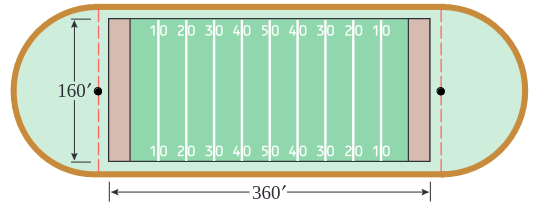
\includegraphics[width=0.7\textwidth]{img/fut.png}
\end{figure}

\begin{enumerate}[label=\alph*)]
\item Demuestre que es posible construir una pista de un cuarto de milla
alrededor del campo de fútbol. [Sugerencia: encuentre la
pista más corta que se puede construir alrededor del campo.]

Para esto, primero podemos construir una fórmula que determine la longitud de la pista considerando
\[
P = 2L + d\pi 
\]
donde $L$ es la longitud de un lado recto y $d$ el diámetro de los semicirculos formado para el lado curvo.\\
Si se hiciera una pista en el borde de la cancha:\\
$L = 360 '$\\
$d=160'$
entonces
\[
P = 2(360) + 160 \pi= 720 + 160\pi \approx 1222.654825 pies
\]
Y ya que 1222.65 pies es menor que 1320, significa que sí es posible construir una pista de esta longitud con medidas más grandes.

\item Sea L la longitud de una recta (en pies) y sea x
la distancia (en pies) entre una lateral del campo y una recta de la pista. Haz una gráfica de L versus x. \\
En este caso, podemos adaptar la formúla anterior, considerando $P=1320$ pies.
\[
1320 = 2L + d\pi  
\]
También podemos saber que el diametro de los semicirculos ahora será de 160' mas dos veces el valor de x.
\[
1320 = 2L + (160+2x)\pi  
\]
Y con esta información podemos despejar el valor de un lado recto L con respecto x
\[
2L = 1320 - (160+2x)\pi  
\]
\[
L =\frac{ 1320 - (160+2x)\pi  }{2} = 660-80 \pi -\pi x 
\]
Graficando la función $L(x) =  660-80 \pi -\pi x $ obtenemos:
\begin{figure}[h]
\centering
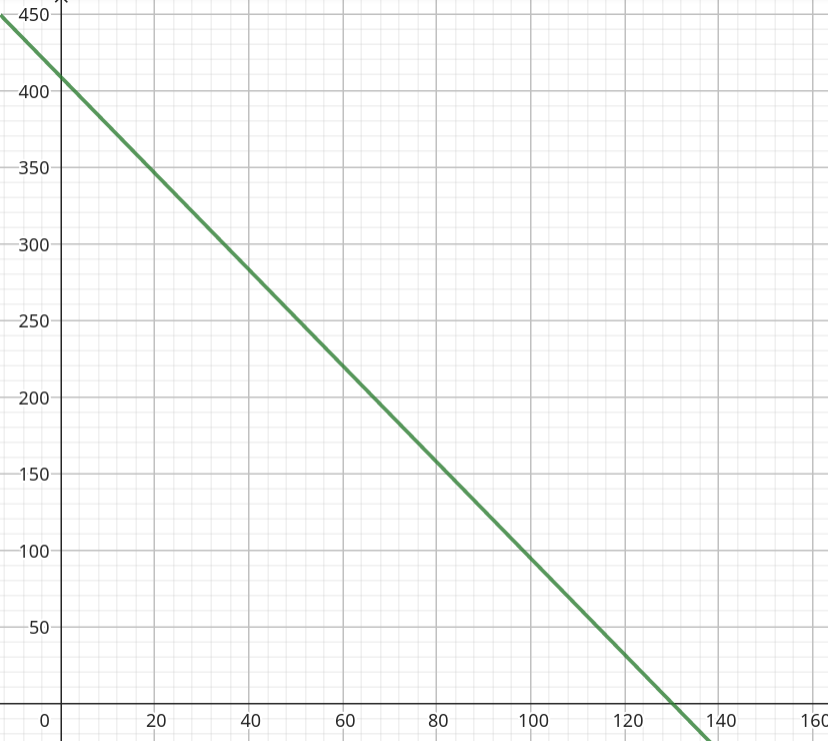
\includegraphics[width=0.7\textwidth]{img/pista.png}
\end{figure}

\item Utilice la gráfica para estimar el valor de x que produce
las rectas más cortas, y luego encuentre este valor de x
exactamente.

El valor más corto de un lado recto debe ser al menos los 360 pies de largo de la cancha, según la gráfica esto se alcanza aproximadamente cuando x vale 15 pies.\\
Para calcular el valor exacto de x a partir del valor de L podemos encontrar la inversa de la función $L(x)$
\[
 L =  660-80 \pi -\pi x 
\]
\[
 L -660 + 80 \pi = -\pi x 
\]
\[
 \frac{L -660 + 80 \pi}{-\pi}  = x 
\]
\[
\therefore L^{-1}(x) = \frac{660-80\pi-L}{\pi} 
\]
Considerando el valor más corto para L es 360 pies sustituimos
\[
x= \frac{660-80\pi-360}{\pi} \approx 15.492965  \; pies 
\]
\item Utilice la gráfica para estimar la longitud de las rectas más largas posibles, y luego encuentre esa longitud exactamente.

La longitud más larga es cuando x vale 0, que en la gráfica se puede interpretar que es aproximadamente 410 pies.\\
Usando la función $L(x) =  660-80 \pi -\pi x$ podemos sustituir el valor de x por 0
\[
L(x) =  660-80 \pi -\pi 0 = 660-80 \pi \approx408.6725 \; pies
\]
\end{enumerate}


\section{Problema 54}
Flores Morán Julieta Melina\\
\\
Una cámara está colocada a x pies de la base de la 
plataforma de lanzamiento de misiles (ver la figura adjunta). Si un misil
de longitud $a$ se lanza verticalmente, demuestre que cuando la base del misil está a $b$ pies por encima de la lente de la cámara, el ángulo $\theta $ subtendido en la lente por el misil es
\[
\theta  = cot ^{-1} \frac{x}{a+b} - cot ^{-1} \frac{x}{b}
\]
\begin{figure}[H]
\centering
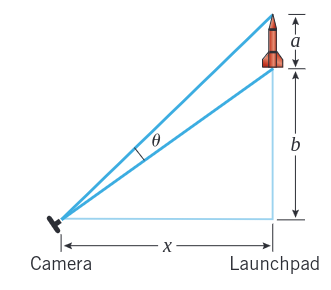
\includegraphics[width=0.5\textwidth]{img/cam.png}
\end{figure}
Podemos interpretar el ángulo $\theta$ como la resta entre los ángulos:
\begin{enumerate}
\item $\beta$, considerándolo el ángulo formado por el triángulo formado por los catetos  x y a+b
\item $\alpha$, considerándolo el ángulo formado por el triángulo formado por los catetos x y b
\end{enumerate}
Entonces, $ \theta = \beta  - \alpha$.
Podemos expresar estos en términos de la cotangente considerando los catetos del triángulo rectángulo que los forman.
\[
cotx= \frac{cateto \; adyacente}{cateto \; opuesto }
\]
\[
cot\beta = \frac{x}{b+a}
\]
\[
cot\alpha = \frac{x}{b}
\]
Entonces, los ángulos $\beta$ y $\alpha$ se pueden calcular con la función inversa de la cotangente $cot^{-1}$
\[
\beta = cot^{-1}\; \frac{x}{a+b}
\]
\[
\alpha = cot^{-1}\;\frac{x}{b}
\]
Y podemos remplazar estos valores por $\alpha$ y $\beta$ en  $ \theta = \beta  - \alpha$, obteniendo que:
\[
 \theta = cot^{-1}\; \frac{x}{a+b}  - cot^{-1}\;\frac{x}{b}
 \]
\begin{figure}[H]
\centering
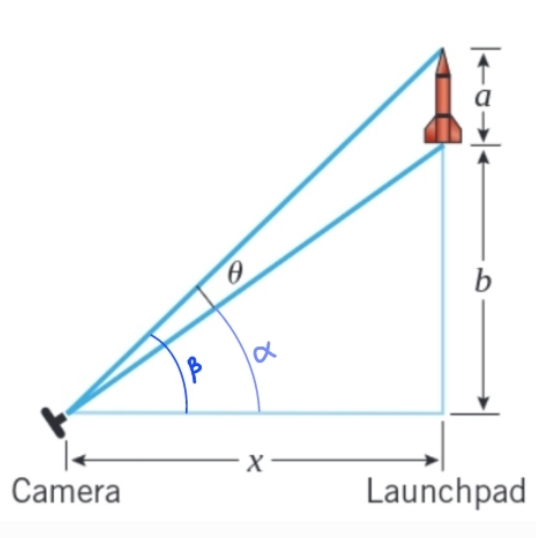
\includegraphics[width=0.5\textwidth]{img/ang.jpg}
\end{figure}


\section{Problema 6}
Zarco Romero José Antonio\\
\\
Una bola de 3 pulgadas de radio está recubierta uniformemente con plástico.
\begin{enumerate}[label=\alph*)]
\item  Exprese el volumen del plástico en función de su espesor.\\
Sea $h$ el espesor del plástico. El volumen del recubrimiento se puede expresar como la diferencia del volumen de la esfera con recubrimiento menos el volumen de la esfera original.
\[
V_{recubrimiento} = V_1 - V_0
\]
\[
V_{recubrimiento} = \frac{4}{3}\pi (r+h)^3 - \frac{4}{3}\pi r^3
\]
Sustituyendo el radio $r=3$pulgadas en la ecuación
\[
V_{recubrimiento} = \frac{4}{3}\pi (3+h)^3 - \frac{4}{3}\pi 3^3
\]
\[
\therefore V_{recubrimiento} = \frac{4}{3}\pi (3+h)^3 - 36\pi
\]

\item  ¿Cuál es el dominio de la función de volumen obtenida en parte (a)?\\
Dado que el espesor no puede ser negativo, entonces
\[
\frac{4}{3}\pi (3+h)^3 - 36\pi \geq 0
\]
\[
\frac{4}{3}\pi (3+h)^3 \geq 36\pi
\]
\[
(3+h)^3 \geq 36\pi \cdot \frac{3}{4\pi}
\]
\[
(3+h)^3 \geq 27
\]
\[
h \geq 0
\]
Además, $h$ no debería exceder el radio de la bola original (3 pulgadas) porque el recubrimiento no puede ser más grueso que el radio de la bola misma.
\[
h \leq 3
\]
$\therefore$ El dominio queda espresado como $[0,3]$
\end{enumerate}

\section{Problema 7}
Zarco Romero José Antonio\\
\\
Se va a hacer una caja de cartón, con la parte superior cerrada a partir de un piso de 6 por 10 pies cortando cuatro cuadrados de igual tamaño (ver la figura adjunta), doblando a lo largo de la línea discontinua
líneas y metiendo las dos solapas adicionales hacia adentro.

\begin{enumerate}[label=\alph*)]
\item Encuentre una fórmula que exprese el volumen de la caja como función de la longitud de los lados de los cuadrados recortados.

Sea $x$ la longitud de cada lado de los cuadrados recortados, las dimensiones de la base quedan expresadas como
\begin{itemize}
	\item Alto $=x$ ft
	\item Ancho $=6-2x$ ft
	\item Largo $=5-x$ ft
\end{itemize}

\begin{figure}[h]
	\centering
	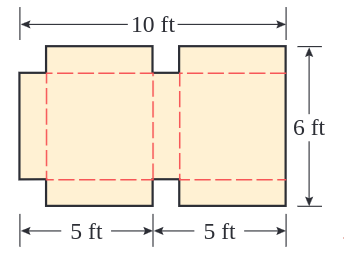
\includegraphics[width=0.5\textwidth]{img/prob7.png}
\end{figure}

Sustituimos los valores en la fórmula para calcular el $Volumen = Largo \cdot Ancho \cdot Alto$
\[
\therefore V(x) = (5-x) \cdot (6-2x) \cdot x \ \  ft^3
\]

\item Encuentre una desigualdad que especifique el dominio de la función en la parte (a).

Dado que la longitud de los lados de los cuadrados recortados $x$ debe recortarse del cartón, $x > 0$. Además, la longitud no puede ser más grande que la mitad de la longitud del lado más corto del cartón, $x < 3$.
\[\therefore 0<x<3\]

\item Utilice la gráfica de la función de volumen para estimar las dimensiones de la caja de mayor volumen.

La gráfica nos dice que la caja de volumen máximo se da para un valor de $x$ que está entre 1 y 2 pies (aproximadamente $x \approx 1.21$ft).

Si $x=1.21$ ft, entonces las dimensiones de la base quedan expresadas como:

\begin{itemize}
	\item Alto $=1.21$ ft
	\item Ancho $=6-2(1.21)=6-2.42=3.58$ ft
	\item Largo $=5-x=5-1.21=3.79$ ft
\end{itemize}

También, muestra que el volumen máximo es de aproximadamente $V \approx 16.41 ft^3$. 

A su vez, muestra que el volumen disminuye hacia cero a medida que x se acerca a 0 o 3.

\begin{figure}[h]
	\centering
	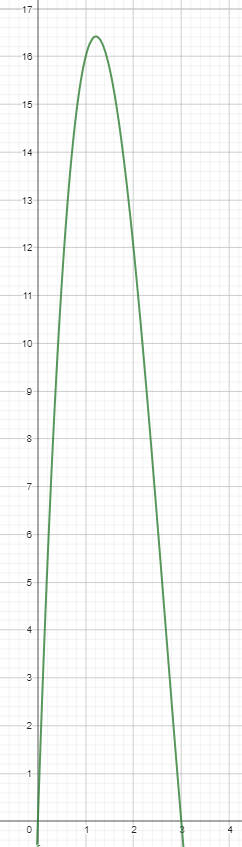
\includegraphics[height=0.6\textheight]{img/p7_vmax.png}
\end{figure}

\end{enumerate}

\section{Problema 22}
Flores Morán Julieta Melina\\
\\
La figura adjunta muestra un modelo para la variación de mareas en una entrada a la Bahía de San Francisco durante un período de 24 horas.
Encuentre una ecuación de la forma $y = y_0 + y_1 sin(at + b)$ para el
modelo, suponiendo que t = 0 corresponde a la medianoche.\\
\begin{figure}[h]
\centering
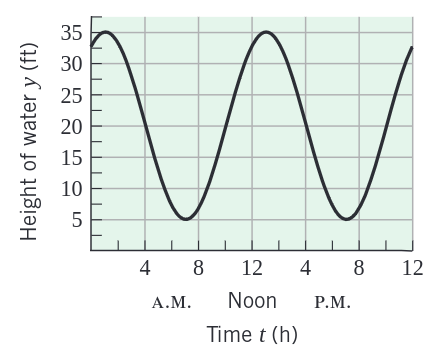
\includegraphics[width=0.5\textwidth]{img/prob22.png}
\end{figure}
Para encontrar la función hay que tener en cuenta la ecuación de la onda ya que es un movimiento oscilatorio.
\[
y = C + A sen (wt+\phi) 
\]
Para esto, hay que calcular los diferentes elementos que la componen. \\ \\
C será el eje sobre el que oscila la onda, es decir, la línea de equilibrio de la onda. En este caso considerando que el punto más bajo es en 5 y el más alto en 35.
\[
C = \frac{35-5}{2} + 5 = \frac{30}{2}+ 5 =15 + 5 = 20
\]
A será la amplitud, de nuevo considerando que 35 es el valor más alto.
\[
A = 35 - 20 = 15
\]
w siendo la frecuencia angular se puede calcular en base al periodo considerando que
\[
T=\frac{2\pi}{w}
\]
\[
\therefore w = \frac{2\pi}{T} 
\]
\[
 w = \frac{2\pi}{12} = \frac{\pi}{6}
\]
$\phi$ siendo la fase, la podemos encontrar en base al desfase de la funsión seno con la dada, que es 10 hacía la derecha, entonces
\[
 w(t+\phi)  = \frac{\pi}{6}(t-10) = \frac{\pi}{6}t+\frac{-10\pi}{6} = \frac{\pi}{6}t-\frac{5\pi}{3} 
\]
Con estos datos obtenemos que: 
\[
y = 20 + 15 sen (\frac{\pi}{6}t-\frac{5\pi}{3}) 
\]

\end{document}